% ============================================================
% Iskole School Management System — Activity Diagrams
% A4 Landscape, swimlane columns, simple tikz styles
% Compile:  pdflatex activity_diagrams.tex
% ============================================================
\documentclass[a4paper,landscape]{article}
\usepackage[a4paper,landscape,top=1.8cm,bottom=1.2cm,
            left=1.2cm,right=1.2cm]{geometry}
\usepackage[dvipsnames,svgnames]{xcolor}
\usepackage{tikz}
\usetikzlibrary{shapes.geometric,arrows.meta,calc}
\usepackage{titlesec}
\usepackage{fancyhdr}

%% ── Colours ─────────────────────────────────────────────────
\definecolor{ColHdr} {RGB}{30,58,138}
\definecolor{ActFill}{RGB}{219,234,254}
\definecolor{ActLine}{RGB}{52,109,219}
\definecolor{SysFill}{RGB}{220,254,220}
\definecolor{SysLine}{RGB}{34,139,34}
\definecolor{DecFill}{RGB}{254,244,220}
\definecolor{DecLine}{RGB}{204,120,0}
\definecolor{SwimBg} {RGB}{240,240,248}

%% ── Simple, flat tikz styles (no optional-arg tricks) ───────
\tikzset{
  nd_start/.style={
    circle, fill=black, minimum size=10pt, inner sep=0pt},
  nd_stop/.style={
    circle, fill=black, draw=black, double, double distance=2pt,
    minimum size=10pt, inner sep=0pt},
  nd_act/.style={
    rectangle, rounded corners=3pt,
    draw=ActLine, fill=ActFill,
    text width=4.9cm, minimum height=0.60cm,
    align=center, font=\footnotesize},
  nd_sys/.style={
    rectangle, rounded corners=3pt,
    draw=SysLine, fill=SysFill,
    text width=4.9cm, minimum height=0.60cm,
    align=center, font=\footnotesize\itshape},
  nd_dec/.style={
    diamond, aspect=2.4,
    draw=DecLine, fill=DecFill,
    text width=2.5cm, align=center,
    font=\footnotesize, inner sep=1pt},
  nd_bar/.style={
    rectangle, fill=black,
    minimum height=4pt, inner sep=0pt},
  arr/.style={-{Stealth[length=5pt,width=4pt]},thick},
  lbl/.style={font=\scriptsize,fill=white,inner sep=1pt},
}

%% ── Page header / footer ────────────────────────────────────
\pagestyle{fancy}\fancyhf{}
\fancyhead[C]{\bfseries\color{ColHdr}%
  Iskole School Management System \textbf{—} Activity Diagrams}
\fancyfoot[C]{\small\thepage}
\renewcommand{\headrulewidth}{1pt}
\renewcommand{\headrule}{%
  \hbox to\headwidth{\color{ColHdr}\leaders\hrule height 1pt\hfill}}
\setlength{\headheight}{16pt}

\titleformat{\section*}[block]
  {\bfseries\large\color{ColHdr}}{}{0pt}{}[{\color{ColHdr}\titlerule}]

%% ── Reusable helpers ────────────────────────────────────────
% \swimbox{x}{ytop}{ybot}{label}
\newcommand{\swimbox}[4]{%
  \fill[SwimBg,rounded corners=4pt]
    (#1-2.6,#2+0.15) rectangle (#1+2.6,#3);
  \node[font=\small\bfseries\color{ColHdr}] at (#1,#2) {#4};
}

%%─────────────────────────────────────────────────────────────
%%  PAGE 1 — USER LOGIN  &  PASSWORD RESET
%%─────────────────────────────────────────────────────────────
\begin{document}
\section*{Diagram 1 \;—\; User Login \& Password Reset}

\begin{center}
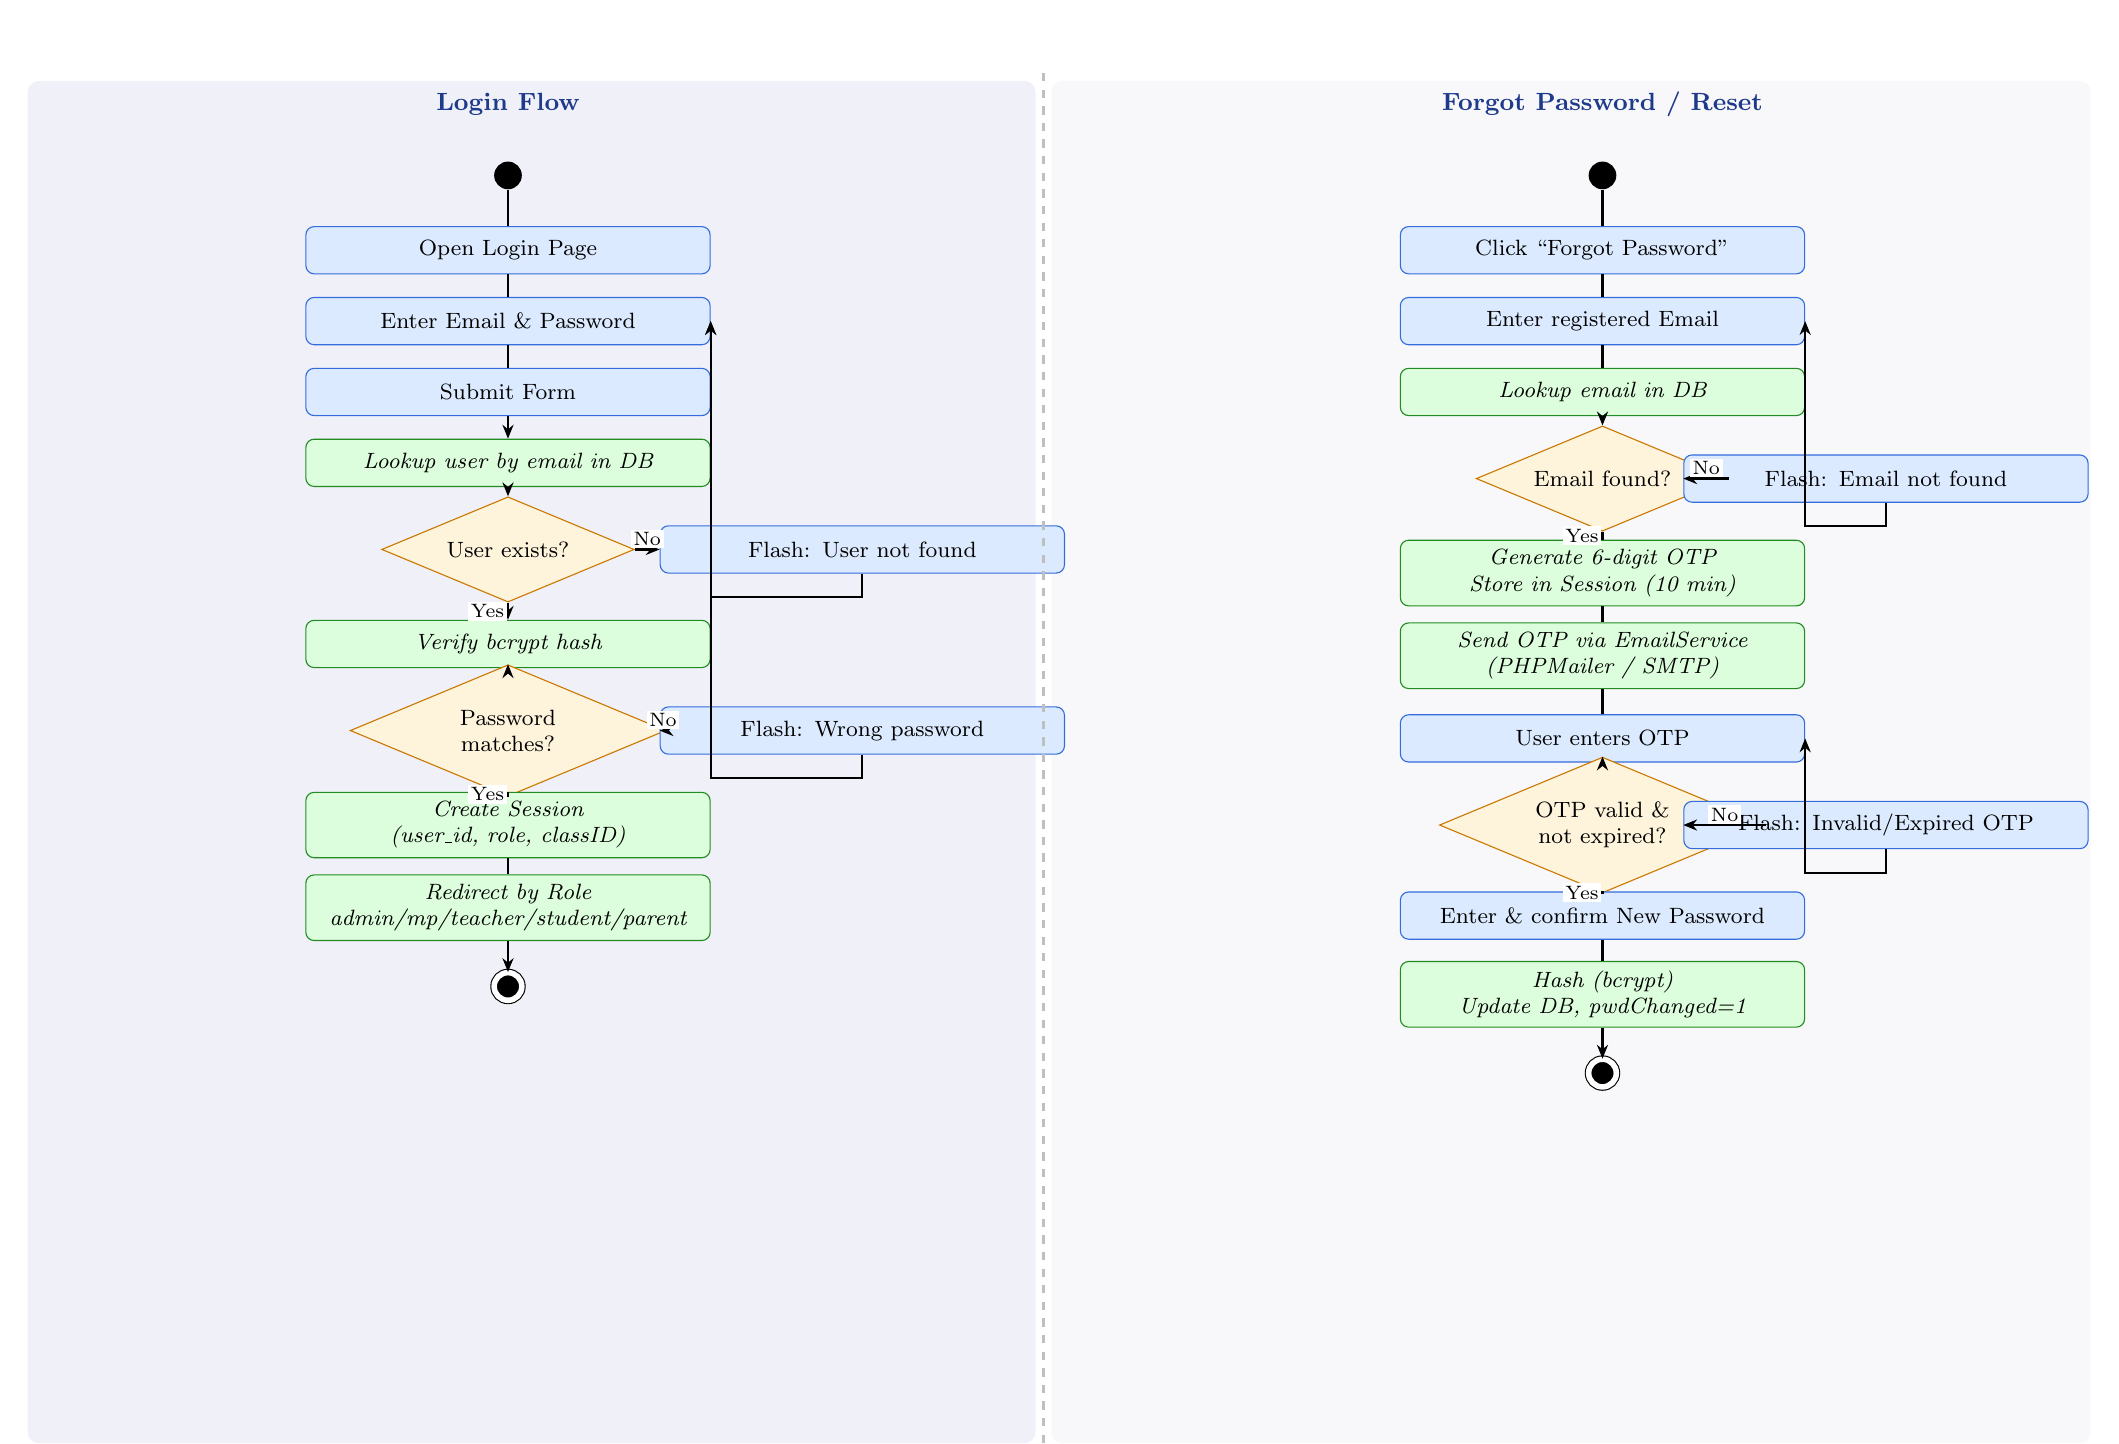
\begin{tikzpicture}[x=1cm,y=1cm]

%% column centres
\def\Lx{6.3} \def\Rx{20.2}

%% backgrounds
\fill[SwimBg,rounded corners=4pt] (0.2,0.5) rectangle (13,-16.8);
\fill[SwimBg!50!white,rounded corners=4pt] (13.2,0.5) rectangle (26.4,-16.8);
\node[font=\small\bfseries\color{ColHdr}] at (\Lx, 0.2)  {Login Flow};
\node[font=\small\bfseries\color{ColHdr}] at (\Rx, 0.2)  {Forgot Password / Reset};

%% ── LEFT: Login ─────────────────────────────────────────────
\node[nd_start] at (\Lx,-0.7)  (LS){};
\node[nd_act]   at (\Lx,-1.65) (L1){Open Login Page};
\node[nd_act]   at (\Lx,-2.55) (L2){Enter Email \& Password};
\node[nd_act]   at (\Lx,-3.45) (L3){Submit Form};
\node[nd_sys]   at (\Lx,-4.35) (L4){Lookup user by email in DB};
\node[nd_dec]   at (\Lx,-5.45) (D1){User exists?};
\node[nd_sys]   at (\Lx,-6.65) (L5){Verify bcrypt hash};
\node[nd_dec]   at (\Lx,-7.75) (D2){Password matches?};
\node[nd_sys]   at (\Lx,-8.95) (L6){Create Session\\(user\_id, role, classID)};
\node[nd_sys]   at (\Lx,-10.0) (L7){Redirect by Role\\admin/mp/teacher/student/parent};
\node[nd_stop]  at (\Lx,-11.0) (LE){};

\node[nd_act] at (\Lx+4.5,-5.45)  (E1){Flash: User not found};
\node[nd_act] at (\Lx+4.5,-7.75)  (E2){Flash: Wrong password};

\draw[arr] (LS)--(L1)--(L2)--(L3)--(L4);
\draw[arr] (L4)--(D1);
\draw[arr] (D1)--node[lbl,left]{Yes}(L5);
\draw[arr] (L5)--(D2);
\draw[arr] (D2)--node[lbl,left]{Yes}(L6)--(L7)--(LE);
\draw[arr] (D1)--node[lbl,above]{No}(E1);
\draw[arr] (D2)--node[lbl,above]{No}(E2);
\draw[arr] (E1.south)--($ (E1.south)+(0,-0.3) $)-|(L2.east);
\draw[arr] (E2.south)--($ (E2.south)+(0,-0.3) $)-|(L2.east);

%% ── RIGHT: Forgot Password ──────────────────────────────────
\node[nd_start] at (\Rx,-0.7)  (RS){};
\node[nd_act]   at (\Rx,-1.65) (R1){Click ``Forgot Password''};
\node[nd_act]   at (\Rx,-2.55) (R2){Enter registered Email};
\node[nd_sys]   at (\Rx,-3.45) (R3){Lookup email in DB};
\node[nd_dec]   at (\Rx,-4.55) (RD1){Email found?};
\node[nd_sys]   at (\Rx,-5.75) (R4){Generate 6-digit OTP\\Store in Session (10 min)};
\node[nd_sys]   at (\Rx,-6.80) (R5){Send OTP via EmailService\\(PHPMailer / SMTP)};
\node[nd_act]   at (\Rx,-7.85) (R6){User enters OTP};
\node[nd_dec]   at (\Rx,-8.95) (RD2){OTP valid \&\\not expired?};
\node[nd_act]   at (\Rx,-10.1) (R7){Enter \& confirm New Password};
\node[nd_sys]   at (\Rx,-11.1) (R8){Hash (bcrypt)\\Update DB, pwdChanged=1};
\node[nd_stop]  at (\Rx,-12.1) (RE){};

\node[nd_act] at (\Rx+3.6,-4.55) (RE1){Flash: Email not found};
\node[nd_act] at (\Rx+3.6,-8.95) (RE2){Flash: Invalid/Expired OTP};

\draw[arr] (RS)--(R1)--(R2)--(R3)--(RD1);
\draw[arr] (RD1)--node[lbl,left]{Yes}(R4)--(R5)--(R6)--(RD2);
\draw[arr] (RD2)--node[lbl,left]{Yes}(R7)--(R8)--(RE);
\draw[arr] (RD1)--node[lbl,above]{No}(RE1);
\draw[arr] (RD2)--node[lbl,above]{No}(RE2);
\draw[arr] (RE1.south)--($(RE1.south)+(0,-0.3)$)-|(R2.east);
\draw[arr] (RE2.south)--($(RE2.south)+(0,-0.3)$)-|(R6.east);

%% divider
\draw[dashed,gray!50,thick] (13.1,0.6)--(13.1,-17);

\end{tikzpicture}
\end{center}

%%─────────────────────────────────────────────────────────────
%%  PAGE 2 — ADMIN WORKFLOW
%%─────────────────────────────────────────────────────────────
\newpage
\section*{Diagram 2 \;—\; Admin Workflow}

\begin{center}
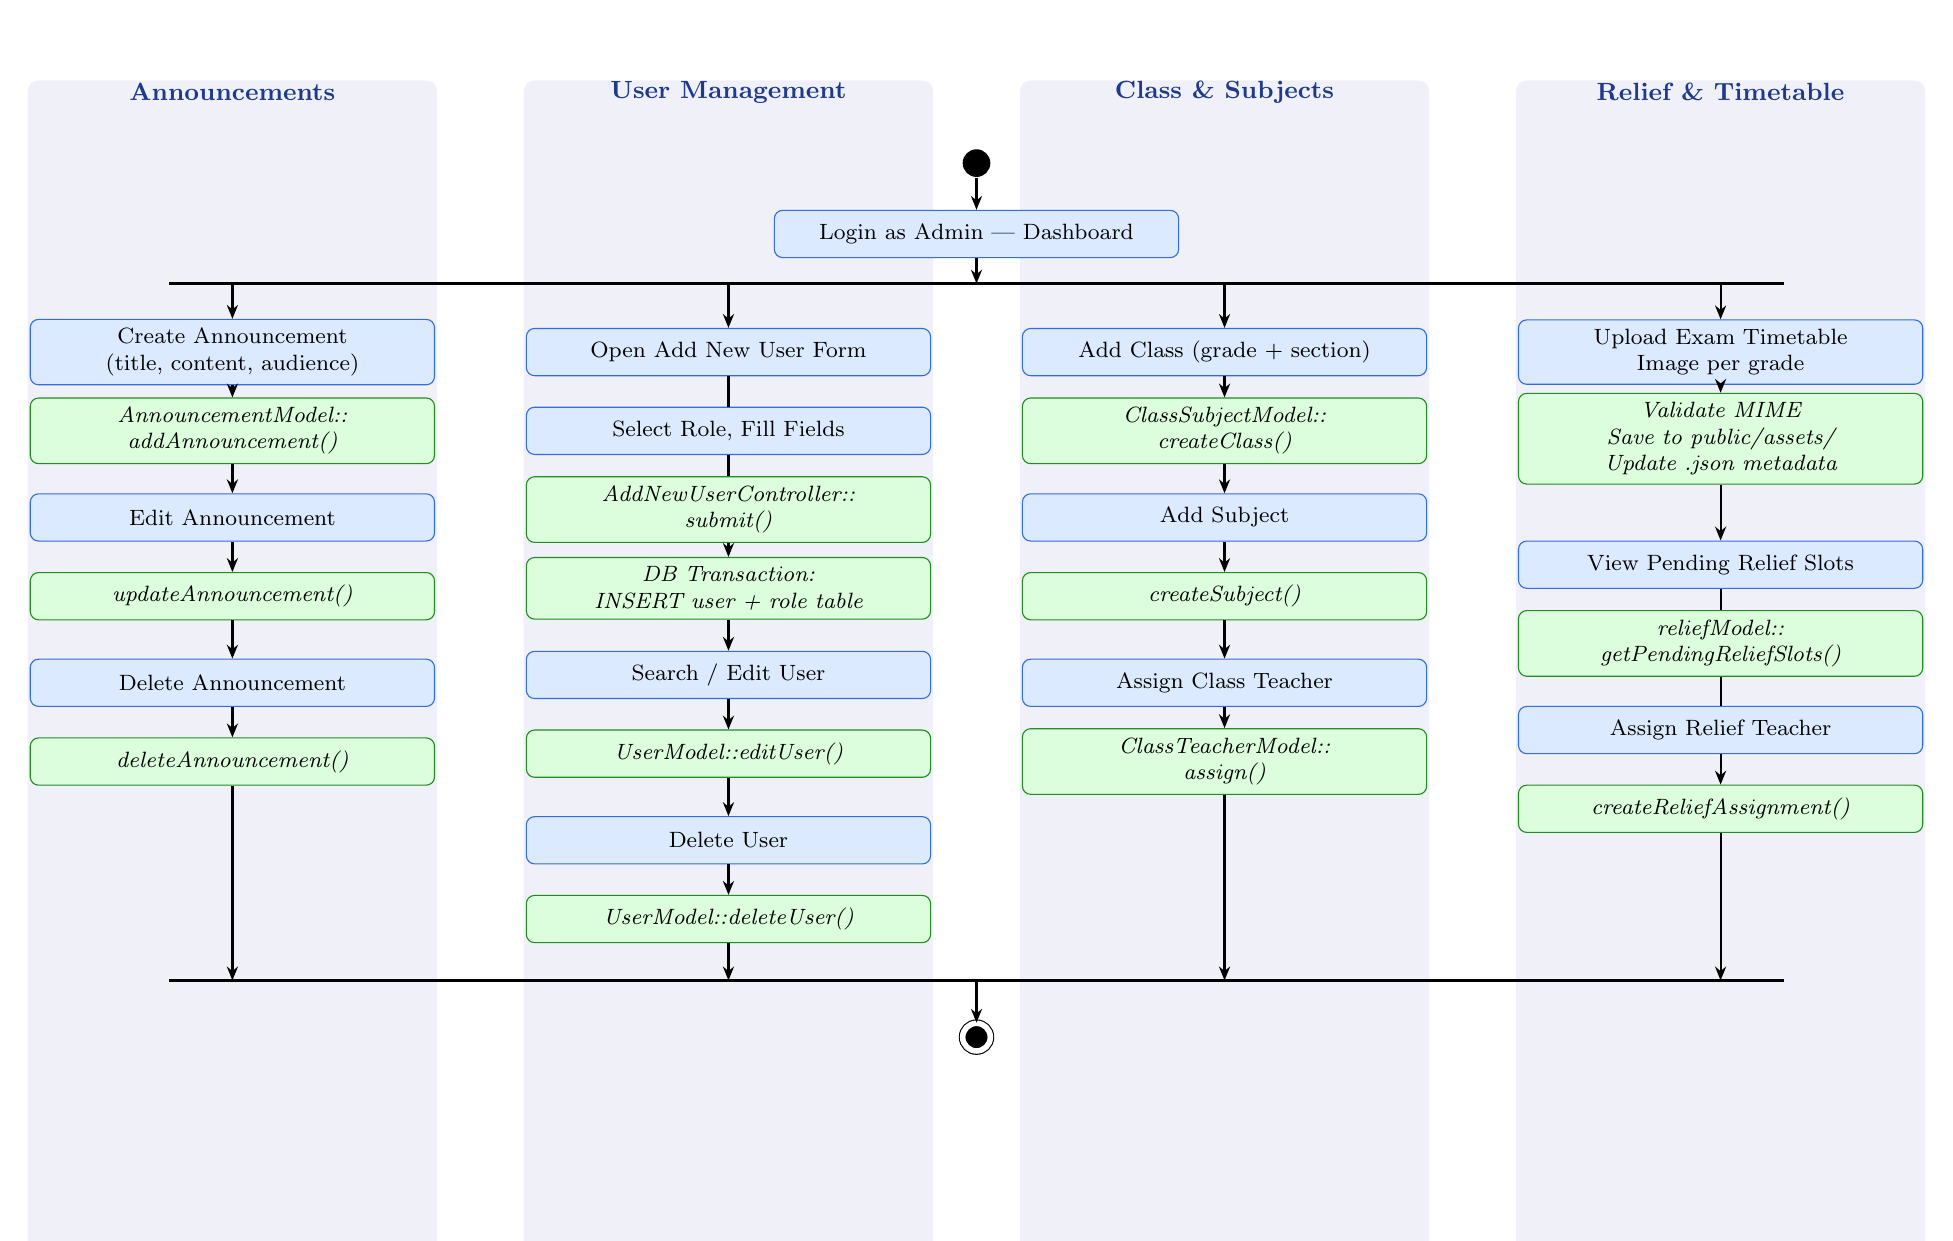
\begin{tikzpicture}[x=1cm,y=1cm]

%% 4 columns:  3.3 | 9.6 | 15.9 | 22.2
\def\cA{3.3}\def\cB{9.6}\def\cC{15.9}\def\cD{22.2}

%% swimlane backgrounds
\swimbox{\cA}{0.2}{-14.6}{Announcements}
\swimbox{\cB}{0.2}{-14.6}{User Management}
\swimbox{\cC}{0.2}{-14.6}{Class \& Subjects}
\swimbox{\cD}{0.2}{-14.6}{Relief \& Timetable}

%% shared header
\node[nd_start]  at (12.75,-0.7)  (S){};
\node[nd_act]    at (12.75,-1.6)  (HD){Login as Admin — Dashboard};
%% fork bar
\fill[black] (2.5,-2.25) rectangle (23.0,-2.21);

%% Col A
\node[nd_act] at (\cA,-3.1)  (A1){Create Announcement\\(title, content, audience)};
\node[nd_sys] at (\cA,-4.1)  (A2){AnnouncementModel::\\addAnnouncement()};
\node[nd_act] at (\cA,-5.2)  (A3){Edit Announcement};
\node[nd_sys] at (\cA,-6.2)  (A4){updateAnnouncement()};
\node[nd_act] at (\cA,-7.3)  (A5){Delete Announcement};
\node[nd_sys] at (\cA,-8.3)  (A6){deleteAnnouncement()};

%% Col B
\node[nd_act] at (\cB,-3.1)  (B1){Open Add New User Form};
\node[nd_act] at (\cB,-4.1)  (B2){Select Role, Fill Fields};
\node[nd_sys] at (\cB,-5.1)  (B3){AddNewUserController::\\submit()};
\node[nd_sys] at (\cB,-6.1)  (B4){DB Transaction:\\INSERT user + role table};
\node[nd_act] at (\cB,-7.2)  (B5){Search / Edit User};
\node[nd_sys] at (\cB,-8.2)  (B6){UserModel::editUser()};
\node[nd_act] at (\cB,-9.3)  (B7){Delete User};
\node[nd_sys] at (\cB,-10.3) (B8){UserModel::deleteUser()};

%% Col C
\node[nd_act] at (\cC,-3.1)  (C1){Add Class (grade + section)};
\node[nd_sys] at (\cC,-4.1)  (C2){ClassSubjectModel::\\createClass()};
\node[nd_act] at (\cC,-5.2)  (C3){Add Subject};
\node[nd_sys] at (\cC,-6.2)  (C4){createSubject()};
\node[nd_act] at (\cC,-7.3)  (C5){Assign Class Teacher};
\node[nd_sys] at (\cC,-8.3)  (C6){ClassTeacherModel::\\assign()};

%% Col D
\node[nd_act] at (\cD,-3.1)  (D1){Upload Exam Timetable\\Image per grade};
\node[nd_sys] at (\cD,-4.2)  (D2){Validate MIME\\Save to public/assets/\\Update .json metadata};
\node[nd_act] at (\cD,-5.8)  (D3){View Pending Relief Slots};
\node[nd_sys] at (\cD,-6.8)  (D4){reliefModel::\\getPendingReliefSlots()};
\node[nd_act] at (\cD,-7.9)  (D5){Assign Relief Teacher};
\node[nd_sys] at (\cD,-8.9)  (D6){createReliefAssignment()};

%% join bar + stop
\fill[black] (2.5,-11.1) rectangle (23.0,-11.06);
\node[nd_stop] at (12.75,-11.8) (E){};

%% arrows
\draw[arr] (S)--(HD);
\draw[arr] (HD.south)--(12.75,-2.23);
\foreach \x/\n in {\cA/A1,\cB/B1,\cC/C1,\cD/D1}
  {\draw[arr] (\x,-2.23)--(\n);}

\draw[arr] (A1)--(A2); \draw[arr] (A3)--(A4); \draw[arr] (A5)--(A6);
\draw[arr] (A2)--(A3); \draw[arr] (A4)--(A5);

\draw[arr] (B1)--(B2)--(B3)--(B4); \draw[arr] (B5)--(B6); \draw[arr] (B7)--(B8);
\draw[arr] (B4)--(B5); \draw[arr] (B6)--(B7);

\draw[arr] (C1)--(C2); \draw[arr] (C3)--(C4); \draw[arr] (C5)--(C6);
\draw[arr] (C2)--(C3); \draw[arr] (C4)--(C5);

\draw[arr] (D1)--(D2); \draw[arr] (D3)--(D4)--(D5)--(D6);
\draw[arr] (D2)--(D3);

\draw[arr] (A6)--(\cA,-11.08);
\draw[arr] (B8)--(\cB,-11.08);
\draw[arr] (C6)--(\cC,-11.08);
\draw[arr] (D6)--(\cD,-11.08);
\draw[arr] (12.75,-11.06)--(E);

\end{tikzpicture}
\end{center}

%%─────────────────────────────────────────────────────────────
%%  PAGE 3 — TEACHER WORKFLOW
%%─────────────────────────────────────────────────────────────
\newpage
\section*{Diagram 3 \;—\; Teacher Workflow}

\begin{center}
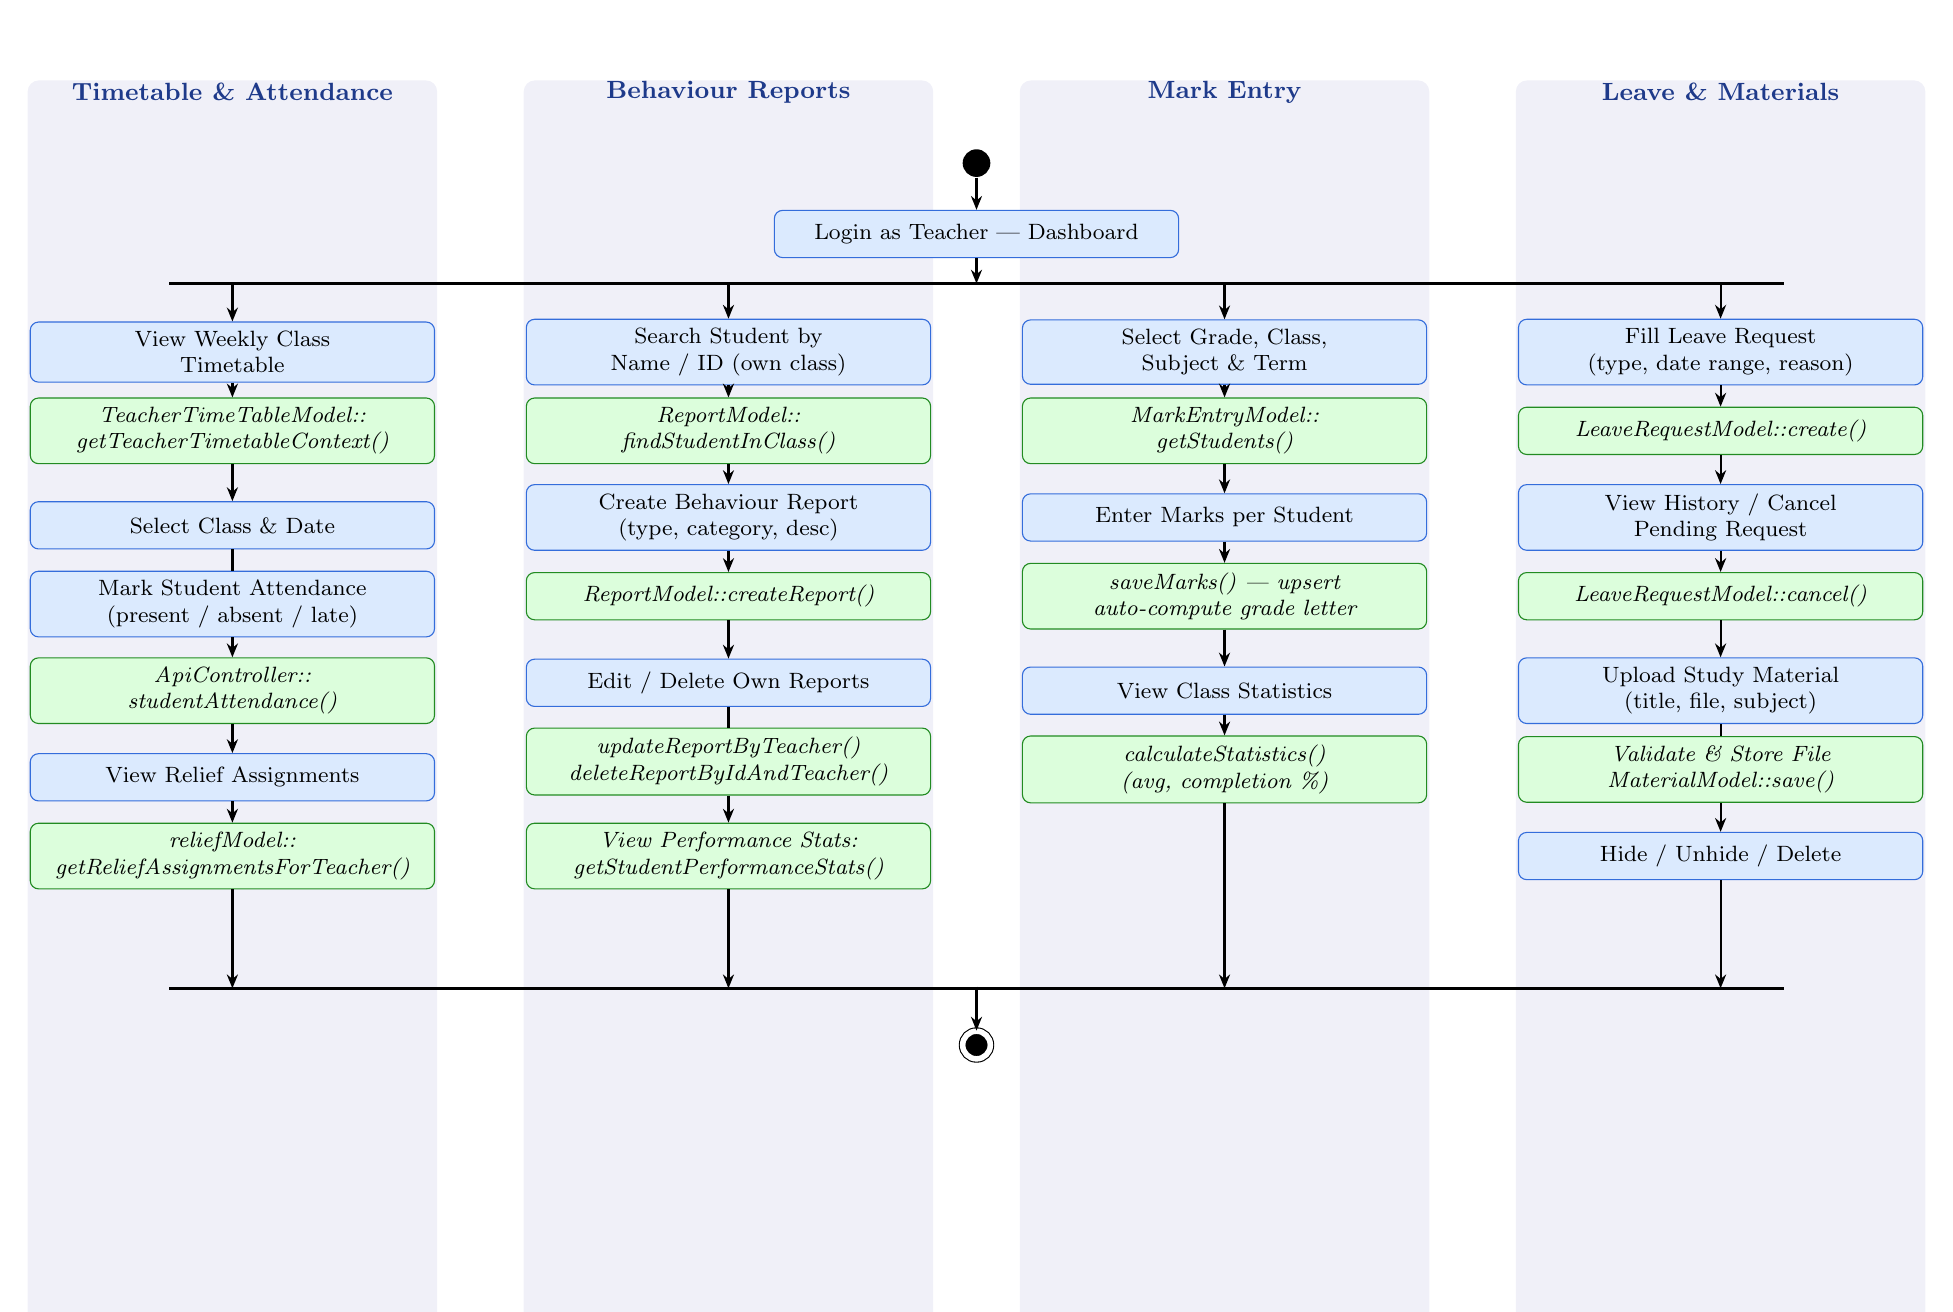
\begin{tikzpicture}[x=1cm,y=1cm]

\def\cA{3.3}\def\cB{9.6}\def\cC{15.9}\def\cD{22.2}

\swimbox{\cA}{0.2}{-15.5}{Timetable \& Attendance}
\swimbox{\cB}{0.2}{-15.5}{Behaviour Reports}
\swimbox{\cC}{0.2}{-15.5}{Mark Entry}
\swimbox{\cD}{0.2}{-15.5}{Leave \& Materials}

\node[nd_start] at (12.75,-0.7)  (S){};
\node[nd_act]   at (12.75,-1.6)  (HD){Login as Teacher — Dashboard};
\fill[black] (2.5,-2.25) rectangle (23.0,-2.21);

%% Col A
\node[nd_act] at (\cA,-3.1)  (A1){View Weekly Class\\Timetable};
\node[nd_sys] at (\cA,-4.1)  (A2){TeacherTimeTableModel::\\getTeacherTimetableContext()};
\node[nd_act] at (\cA,-5.3)  (A3){Select Class \& Date};
\node[nd_act] at (\cA,-6.3)  (A4){Mark Student Attendance\\(present / absent / late)};
\node[nd_sys] at (\cA,-7.4)  (A5){ApiController::\\studentAttendance()};
\node[nd_act] at (\cA,-8.5)  (A6){View Relief Assignments};
\node[nd_sys] at (\cA,-9.5)  (A7){reliefModel::\\getReliefAssignmentsForTeacher()};

%% Col B
\node[nd_act] at (\cB,-3.1)  (B1){Search Student by\\Name / ID (own class)};
\node[nd_sys] at (\cB,-4.1)  (B2){ReportModel::\\findStudentInClass()};
\node[nd_act] at (\cB,-5.2)  (B3){Create Behaviour Report\\(type, category, desc)};
\node[nd_sys] at (\cB,-6.2)  (B4){ReportModel::createReport()};
\node[nd_act] at (\cB,-7.3)  (B5){Edit / Delete Own Reports};
\node[nd_sys] at (\cB,-8.3)  (B6){updateReportByTeacher()\\deleteReportByIdAndTeacher()};
\node[nd_sys] at (\cB,-9.5)  (B7){View Performance Stats:\\getStudentPerformanceStats()};

%% Col C
\node[nd_act] at (\cC,-3.1)  (C1){Select Grade, Class,\\Subject \& Term};
\node[nd_sys] at (\cC,-4.1)  (C2){MarkEntryModel::\\getStudents()};
\node[nd_act] at (\cC,-5.2)  (C3){Enter Marks per Student};
\node[nd_sys] at (\cC,-6.2)  (C4){saveMarks() — upsert\\auto-compute grade letter};
\node[nd_act] at (\cC,-7.4)  (C5){View Class Statistics};
\node[nd_sys] at (\cC,-8.4)  (C6){calculateStatistics()\\(avg, completion \%)};

%% Col D
\node[nd_act] at (\cD,-3.1)  (D1){Fill Leave Request\\(type, date range, reason)};
\node[nd_sys] at (\cD,-4.1)  (D2){LeaveRequestModel::create()};
\node[nd_act] at (\cD,-5.2)  (D3){View History / Cancel\\Pending Request};
\node[nd_sys] at (\cD,-6.2)  (D4){LeaveRequestModel::cancel()};
\node[nd_act] at (\cD,-7.4)  (D5){Upload Study Material\\(title, file, subject)};
\node[nd_sys] at (\cD,-8.4)  (D6){Validate \& Store File\\MaterialModel::save()};
\node[nd_act] at (\cD,-9.5)  (D7){Hide / Unhide / Delete};

\fill[black] (2.5,-11.2) rectangle (23.0,-11.16);
\node[nd_stop] at (12.75,-11.9) (E){};

\draw[arr] (S)--(HD);
\draw[arr] (HD.south)--(12.75,-2.23);
\foreach \x/\n in {\cA/A1,\cB/B1,\cC/C1,\cD/D1}
  {\draw[arr] (\x,-2.23)--(\n);}

\draw[arr] (A1)--(A2); \draw[arr] (A3)--(A4)--(A5); \draw[arr] (A6)--(A7);
\draw[arr] (A2)--(A3); \draw[arr] (A5)--(A6);

\draw[arr] (B1)--(B2); \draw[arr] (B3)--(B4); \draw[arr] (B5)--(B6)--(B7);
\draw[arr] (B2)--(B3); \draw[arr] (B4)--(B5);

\draw[arr] (C1)--(C2); \draw[arr] (C3)--(C4); \draw[arr] (C5)--(C6);
\draw[arr] (C2)--(C3); \draw[arr] (C4)--(C5);

\draw[arr] (D1)--(D2); \draw[arr] (D3)--(D4); \draw[arr] (D5)--(D6)--(D7);
\draw[arr] (D2)--(D3); \draw[arr] (D4)--(D5);

\draw[arr] (A7)--(\cA,-11.18);
\draw[arr] (B7)--(\cB,-11.18);
\draw[arr] (C6)--(\cC,-11.18);
\draw[arr] (D7)--(\cD,-11.18);
\draw[arr] (12.75,-11.16)--(E);

\end{tikzpicture}
\end{center}

%%─────────────────────────────────────────────────────────────
%%  PAGE 4 — STUDENT WORKFLOW
%%─────────────────────────────────────────────────────────────
\newpage
\section*{Diagram 4 \;—\; Student Workflow}

\begin{center}
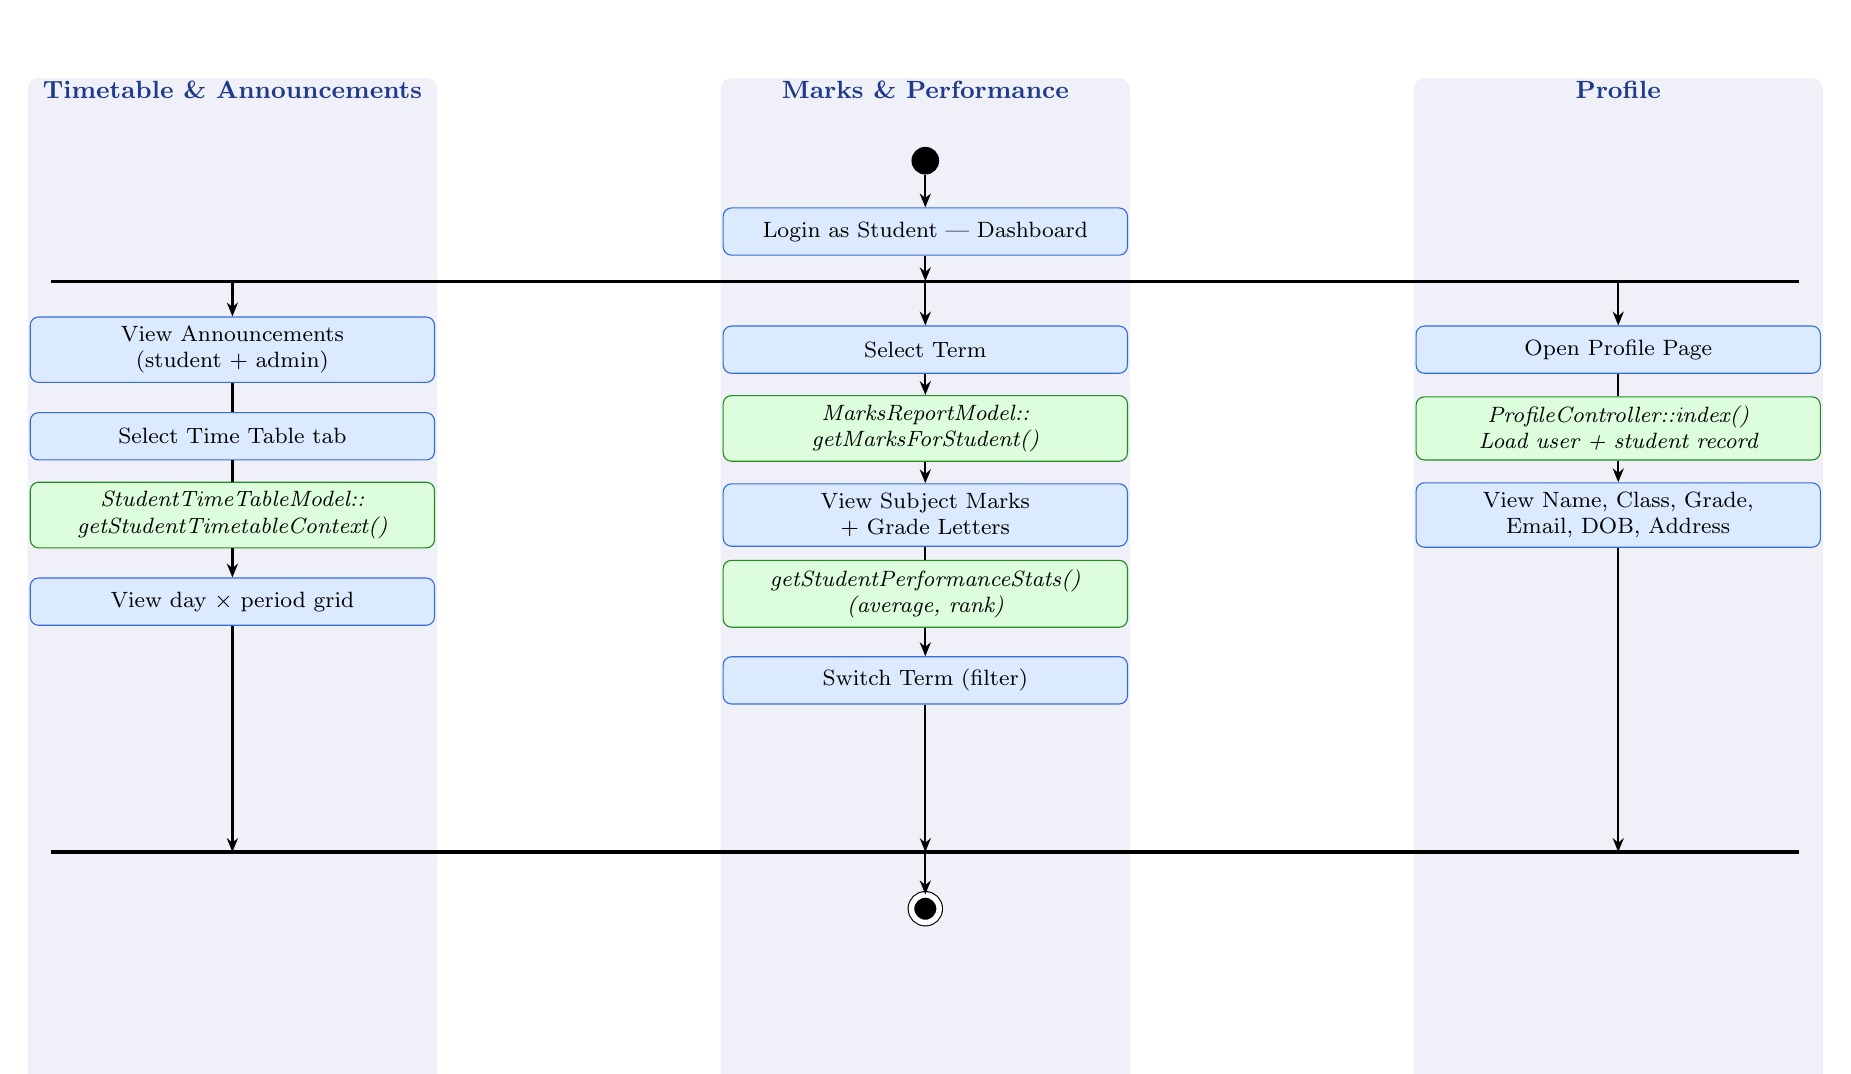
\begin{tikzpicture}[x=1cm,y=1cm]

\def\cA{4.5}\def\cB{13.3}\def\cC{22.1}

\swimbox{\cA}{0.2}{-12.5}{Timetable \& Announcements}
\swimbox{\cB}{0.2}{-12.5}{Marks \& Performance}
\swimbox{\cC}{0.2}{-12.5}{Profile}

\node[nd_start] at (13.3,-0.7)  (S){};
\node[nd_act]   at (13.3,-1.6)  (HD){Login as Student — Dashboard};
\fill[black] (2.2,-2.25) rectangle (24.4,-2.21);

%% Col A
\node[nd_act] at (\cA,-3.1)  (A1){View Announcements\\(student + admin)};
\node[nd_act] at (\cA,-4.2)  (A2){Select Time Table tab};
\node[nd_sys] at (\cA,-5.2)  (A3){StudentTimeTableModel::\\getStudentTimetableContext()};
\node[nd_act] at (\cA,-6.3)  (A4){View day $\times$ period grid};

%% Col B
\node[nd_act] at (\cB,-3.1)  (B1){Select Term};
\node[nd_sys] at (\cB,-4.1)  (B2){MarksReportModel::\\getMarksForStudent()};
\node[nd_act] at (\cB,-5.2)  (B3){View Subject Marks\\+ Grade Letters};
\node[nd_sys] at (\cB,-6.2)  (B4){getStudentPerformanceStats()\\(average, rank)};
\node[nd_act] at (\cB,-7.3)  (B5){Switch Term (filter)};

%% Col C
\node[nd_act] at (\cC,-3.1)  (C1){Open Profile Page};
\node[nd_sys] at (\cC,-4.1)  (C2){ProfileController::index()\\Load user + student record};
\node[nd_act] at (\cC,-5.2)  (C3){View Name, Class, Grade,\\Email, DOB, Address};

\fill[black] (2.2,-9.5) rectangle (24.4,-9.46);
\node[nd_stop] at (13.3,-10.2) (E){};

\draw[arr] (S)--(HD);
\draw[arr] (HD.south)--(13.3,-2.23);
\foreach \x/\n in {\cA/A1,\cB/B1,\cC/C1}
  {\draw[arr] (\x,-2.23)--(\n);}

\draw[arr] (A1)--(A2)--(A3)--(A4);
\draw[arr] (B1)--(B2); \draw[arr] (B3)--(B4)--(B5);
\draw[arr] (B2)--(B3);
\draw[arr] (C1)--(C2)--(C3);

\draw[arr] (A4)--(\cA,-9.48);
\draw[arr] (B5)--(\cB,-9.48);
\draw[arr] (C3)--(\cC,-9.48);
\draw[arr] (13.3,-9.46)--(E);

\end{tikzpicture}
\end{center}

%%─────────────────────────────────────────────────────────────
%%  PAGE 5 — PARENT WORKFLOW
%%─────────────────────────────────────────────────────────────
\newpage
\section*{Diagram 5 \;—\; Parent Workflow}

\begin{center}
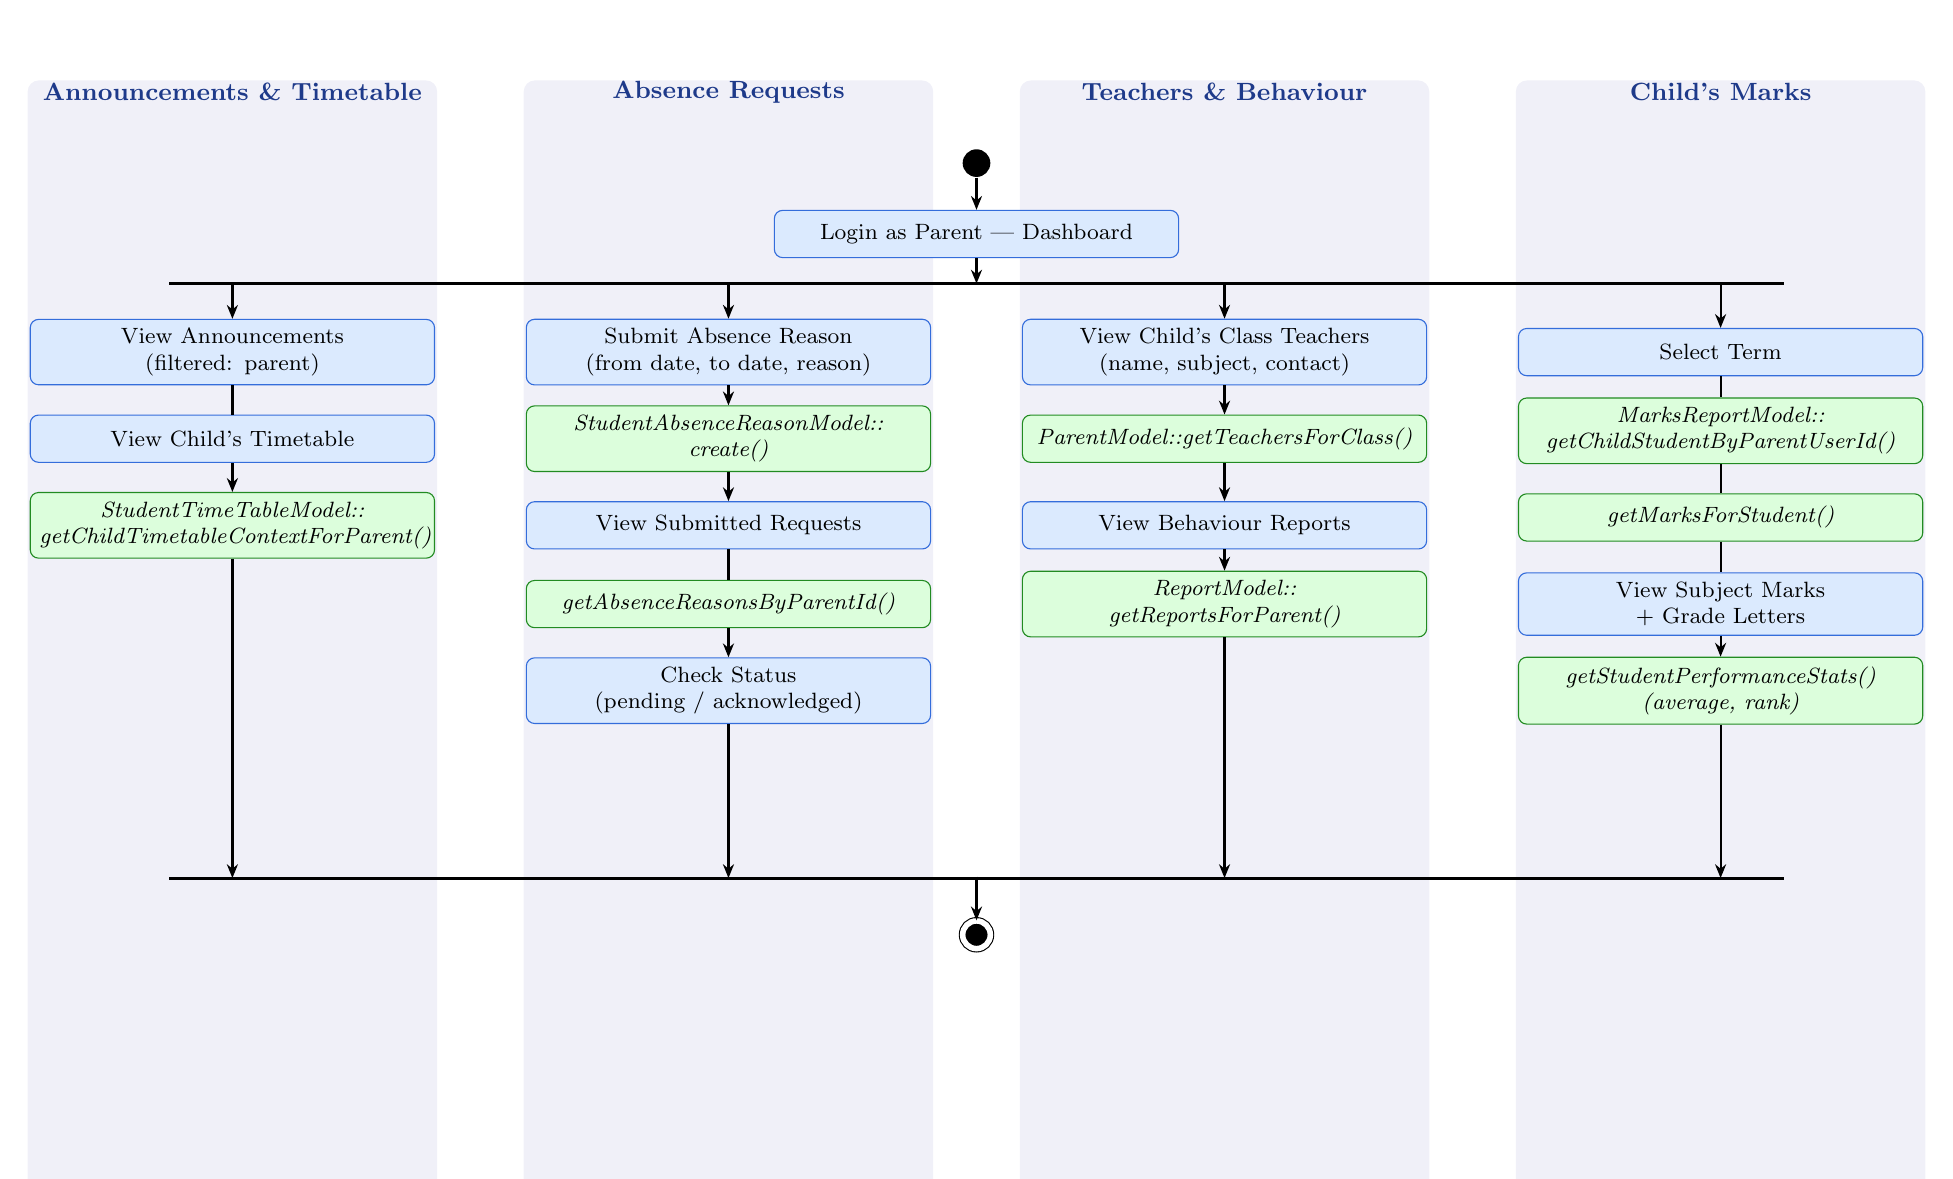
\begin{tikzpicture}[x=1cm,y=1cm]

\def\cA{3.3}\def\cB{9.6}\def\cC{15.9}\def\cD{22.2}

\swimbox{\cA}{0.2}{-13.8}{Announcements \& Timetable}
\swimbox{\cB}{0.2}{-13.8}{Absence Requests}
\swimbox{\cC}{0.2}{-13.8}{Teachers \& Behaviour}
\swimbox{\cD}{0.2}{-13.8}{Child's Marks}

\node[nd_start] at (12.75,-0.7)  (S){};
\node[nd_act]   at (12.75,-1.6)  (HD){Login as Parent — Dashboard};
\fill[black] (2.5,-2.25) rectangle (23.0,-2.21);

%% Col A
\node[nd_act] at (\cA,-3.1)  (A1){View Announcements\\(filtered: parent)};
\node[nd_act] at (\cA,-4.2)  (A2){View Child's Timetable};
\node[nd_sys] at (\cA,-5.3)  (A3){StudentTimeTableModel::\\getChildTimetableContextForParent()};

%% Col B
\node[nd_act] at (\cB,-3.1)  (B1){Submit Absence Reason\\(from date, to date, reason)};
\node[nd_sys] at (\cB,-4.2)  (B2){StudentAbsenceReasonModel::\\create()};
\node[nd_act] at (\cB,-5.3)  (B3){View Submitted Requests};
\node[nd_sys] at (\cB,-6.3)  (B4){getAbsenceReasonsByParentId()};
\node[nd_act] at (\cB,-7.4)  (B5){Check Status\\(pending / acknowledged)};

%% Col C
\node[nd_act] at (\cC,-3.1)  (C1){View Child's Class Teachers\\(name, subject, contact)};
\node[nd_sys] at (\cC,-4.2)  (C2){ParentModel::getTeachersForClass()};
\node[nd_act] at (\cC,-5.3)  (C3){View Behaviour Reports};
\node[nd_sys] at (\cC,-6.3)  (C4){ReportModel::\\getReportsForParent()};

%% Col D
\node[nd_act] at (\cD,-3.1)  (D1){Select Term};
\node[nd_sys] at (\cD,-4.1)  (D2){MarksReportModel::\\getChildStudentByParentUserId()};
\node[nd_sys] at (\cD,-5.2)  (D3){getMarksForStudent()};
\node[nd_act] at (\cD,-6.3)  (D4){View Subject Marks\\+ Grade Letters};
\node[nd_sys] at (\cD,-7.4)  (D5){getStudentPerformanceStats()\\(average, rank)};

\fill[black] (2.5,-9.8) rectangle (23.0,-9.76);
\node[nd_stop] at (12.75,-10.5) (E){};

\draw[arr] (S)--(HD);
\draw[arr] (HD.south)--(12.75,-2.23);
\foreach \x/\n in {\cA/A1,\cB/B1,\cC/C1,\cD/D1}
  {\draw[arr] (\x,-2.23)--(\n);}

\draw[arr] (A1)--(A2)--(A3);
\draw[arr] (B1)--(B2); \draw[arr] (B3)--(B4)--(B5); \draw[arr] (B2)--(B3);
\draw[arr] (C1)--(C2); \draw[arr] (C3)--(C4);       \draw[arr] (C2)--(C3);
\draw[arr] (D1)--(D2)--(D3)--(D4)--(D5);

\draw[arr] (A3)--(\cA,-9.78);
\draw[arr] (B5)--(\cB,-9.78);
\draw[arr] (C4)--(\cC,-9.78);
\draw[arr] (D5)--(\cD,-9.78);
\draw[arr] (12.75,-9.76)--(E);

\end{tikzpicture}
\end{center}

%%─────────────────────────────────────────────────────────────
%%  PAGE 6 — MP / MANAGER WORKFLOW
%%─────────────────────────────────────────────────────────────
\newpage
\section*{Diagram 6 \;—\; MP / Manager Workflow}

\begin{center}
\begin{tikzpicture}[x=1cm,y=1cm]

\def\cA{3.3}\def\cB{9.6}\def\cC{15.9}\def\cD{22.2}

\swimbox{\cA}{0.2}{-14.8}{Announcements}
\swimbox{\cB}{0.2}{-14.8}{Leave Approval}
\swimbox{\cC}{0.2}{-14.8}{Teacher Attendance}
\swimbox{\cD}{0.2}{-14.8}{Academic Overview}

\node[nd_start] at (12.75,-0.7)  (S){};
\node[nd_act]   at (12.75,-1.6)  (HD){Login as Manager (MP) — Dashboard};
\fill[black] (2.5,-2.25) rectangle (23.0,-2.21);

%% Col A
\node[nd_act] at (\cA,-3.1)  (A1){Create Announcement\\(title, content, audience)};
\node[nd_sys] at (\cA,-4.2)  (A2){AnnouncementModel::\\addAnnouncement()};
\node[nd_act] at (\cA,-5.3)  (A3){Edit Announcement};
\node[nd_sys] at (\cA,-6.3)  (A4){updateAnnouncement()};
\node[nd_act] at (\cA,-7.4)  (A5){Delete Announcement};
\node[nd_sys] at (\cA,-8.4)  (A6){deleteAnnouncement()};

%% Col B
\node[nd_sys] at (\cB,-3.1)  (B1){LeaveRequestModel::\\getPending()};
\node[nd_act] at (\cB,-4.2)  (B2){Review Request\\(teacher, type, dates)};
\node[nd_dec] at (\cB,-5.5)  (BD){Approve?};
\node[nd_sys] at (\cB,-6.9)  (B3){updateStatus('approved',\\comment)};
\node[nd_sys] at ($ (\cB)+(3.0,-6.9) $) (B4){updateStatus('rejected',\\comment)};

%% Col C
\node[nd_act] at (\cC,-3.1)  (C1){Select Date};
\node[nd_sys] at (\cC,-4.1)  (C2){Load all Teachers};
\node[nd_act] at (\cC,-5.2)  (C3){Mark each Teacher:\\present / absent / leave};
\node[nd_sys] at (\cC,-6.3)  (C4){ApiController::\\teacherAttendance()\\(bulk upsert)};
\node[nd_act] at (\cC,-7.7)  (C5){Check Pending Relief Slots};
\node[nd_sys] at (\cC,-8.7)  (C6){reliefModel::\\getPendingReliefSlots()};

%% Col D
\node[nd_act] at (\cD,-3.1)  (D1){Open Academic Overview\\(public, no auth)};
\node[nd_sys] at (\cD,-4.2)  (D2){AcademicOverviewController::\\index()};
\node[nd_act] at (\cD,-5.3)  (D3){View school-wide stats,\\class lists, schedules};

\fill[black] (2.5,-11.0) rectangle (23.0,-10.96);
\node[nd_stop] at (12.75,-11.7) (E){};

\draw[arr] (S)--(HD);
\draw[arr] (HD.south)--(12.75,-2.23);
\foreach \x/\n in {\cA/A1,\cB/B1,\cC/C1,\cD/D1}
  {\draw[arr] (\x,-2.23)--(\n);}

\draw[arr] (A1)--(A2); \draw[arr] (A3)--(A4); \draw[arr] (A5)--(A6);
\draw[arr] (A2)--(A3); \draw[arr] (A4)--(A5);

\draw[arr] (B1)--(B2)--(BD);
\draw[arr] (BD)--node[lbl,left]{Yes}(B3);
\draw[arr] (BD)--node[lbl,above]{No}(B4);

\draw[arr] (C1)--(C2)--(C3)--(C4); \draw[arr] (C5)--(C6);
\draw[arr] (C4)--(C5);

\draw[arr] (D1)--(D2)--(D3);

%% column bottoms to join
\draw[arr] (A6)--(\cA,-10.98);
\draw[arr] (B3)--(\cB,-10.98);
\draw[arr] (B4.south)--($(B4.south)+(0,-0.3)$)--($(\cB,-10.98)+(3.0,0)$)--(\cB,-10.98);
\draw[arr] (C6)--(\cC,-10.98);
\draw[arr] (D3)--(\cD,-10.98);
\draw[arr] (12.75,-10.96)--(E);

\end{tikzpicture}
\end{center}

%%─────────────────────────────────────────────────────────────
%%  LEGEND (last page)
%%─────────────────────────────────────────────────────────────
\newpage
\section*{Legend}
\begin{center}
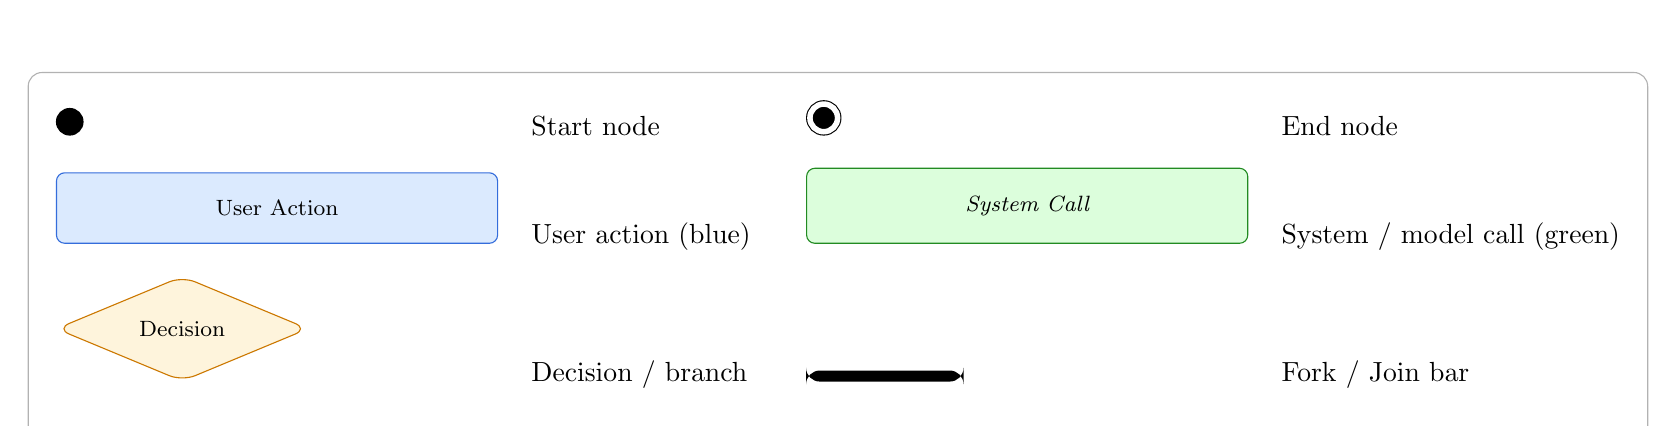
\begin{tikzpicture}[x=1cm,y=1cm]
\node[draw=gray!60,rounded corners=5pt,fill=white,inner sep=10pt] at (0,0) {%
  \begin{tabular}{@{}ll@{\quad\quad}ll@{}}
    \tikz{\node[nd_start]{};} & Start node
    & \tikz{\node[nd_stop]{};} & End node \\[8pt]
    \tikz{\node[nd_act]{User Action};} & User action (blue)
    & \tikz{\node[nd_sys]{System Call};} & System / model call (green) \\[8pt]
    \tikz{\node[nd_dec]{Decision};} & Decision / branch
    & \tikz{\fill[black](0,0) rectangle (2cm,4pt);} & Fork / Join bar \\[8pt]
  \end{tabular}%
};
\end{tikzpicture}
\end{center}

\end{document}
